\documentclass[main.tex]{subfiles}
\begin{document}
	\chapter{結果}
	
	\section{outflowの確認}
	
	\begin{figure}[htbp]
		\centering
		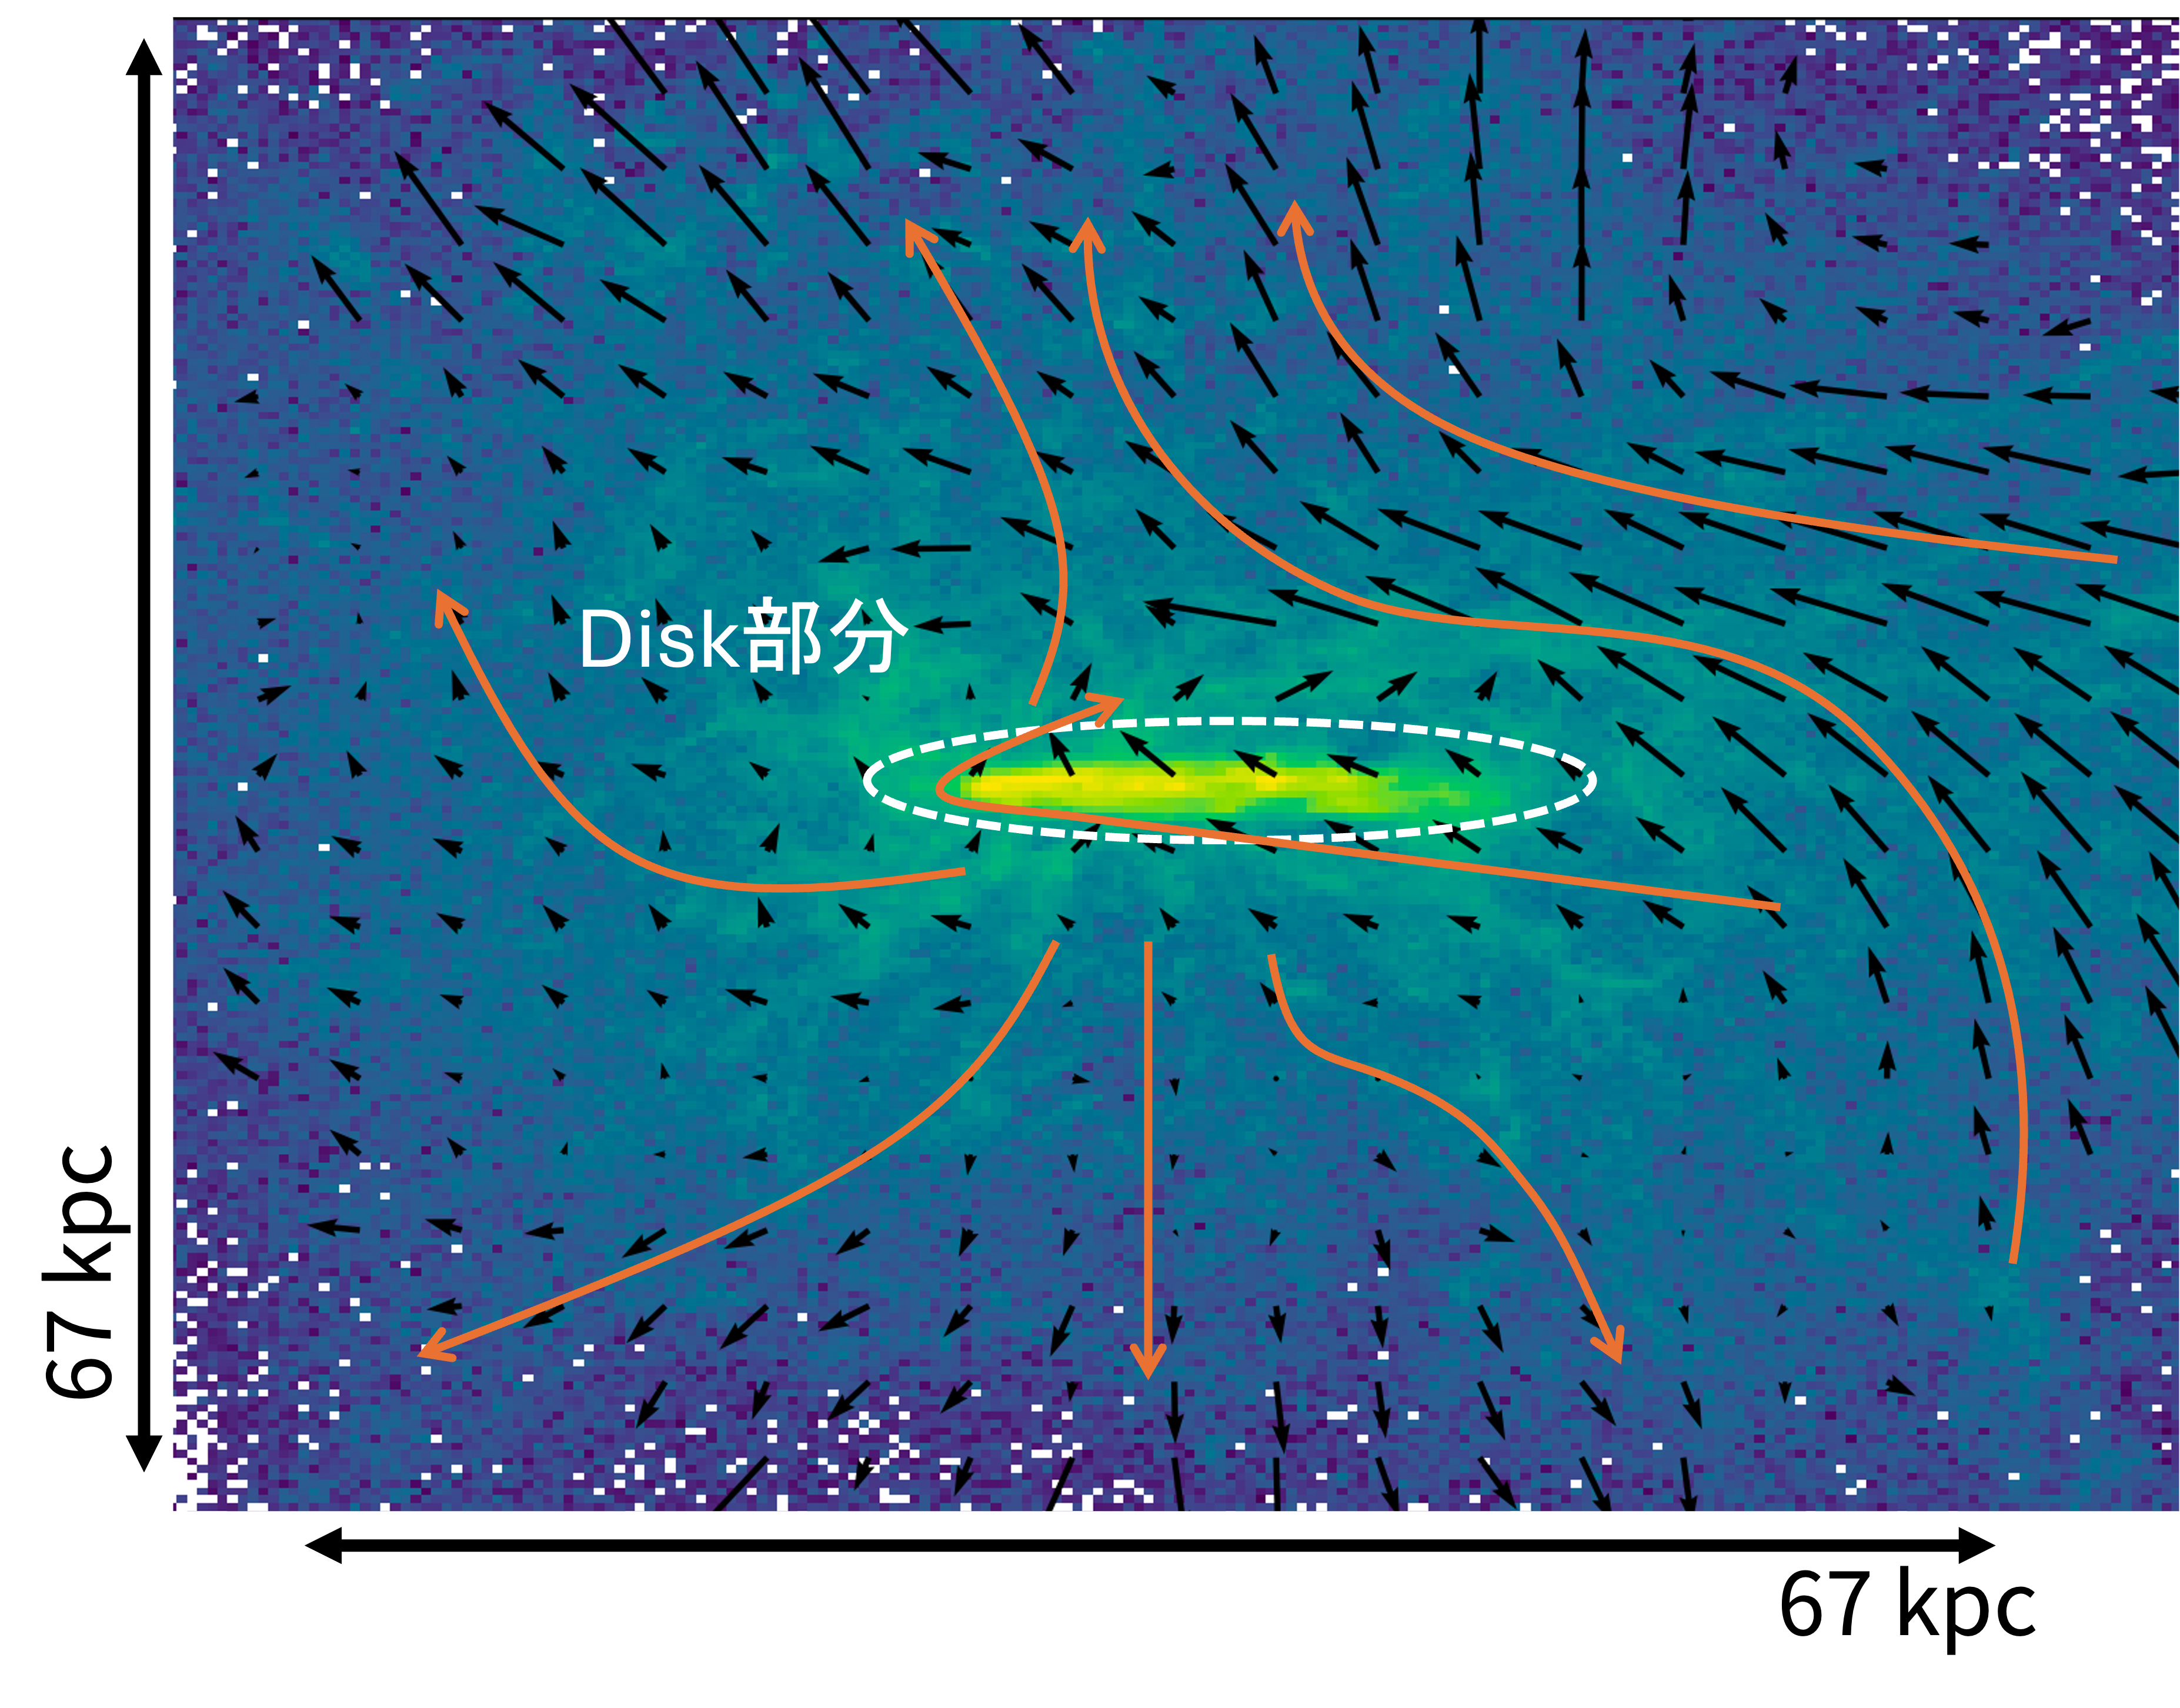
\includegraphics[width=0.6\linewidth]{pic/outflow_subhalo342447}
		\captionsetup{width=.8\linewidth}
		\caption{subhalo342447をedge-onで表示したもの.Massesを背景に表示して速度場を表示している.}
		\label{fig:outflowsubhalo342447}
	\end{figure}
	
	\begin{figure}[htbp]
		\centering
		\begin{minipage}[b]{0.45\linewidth}
			\centering
			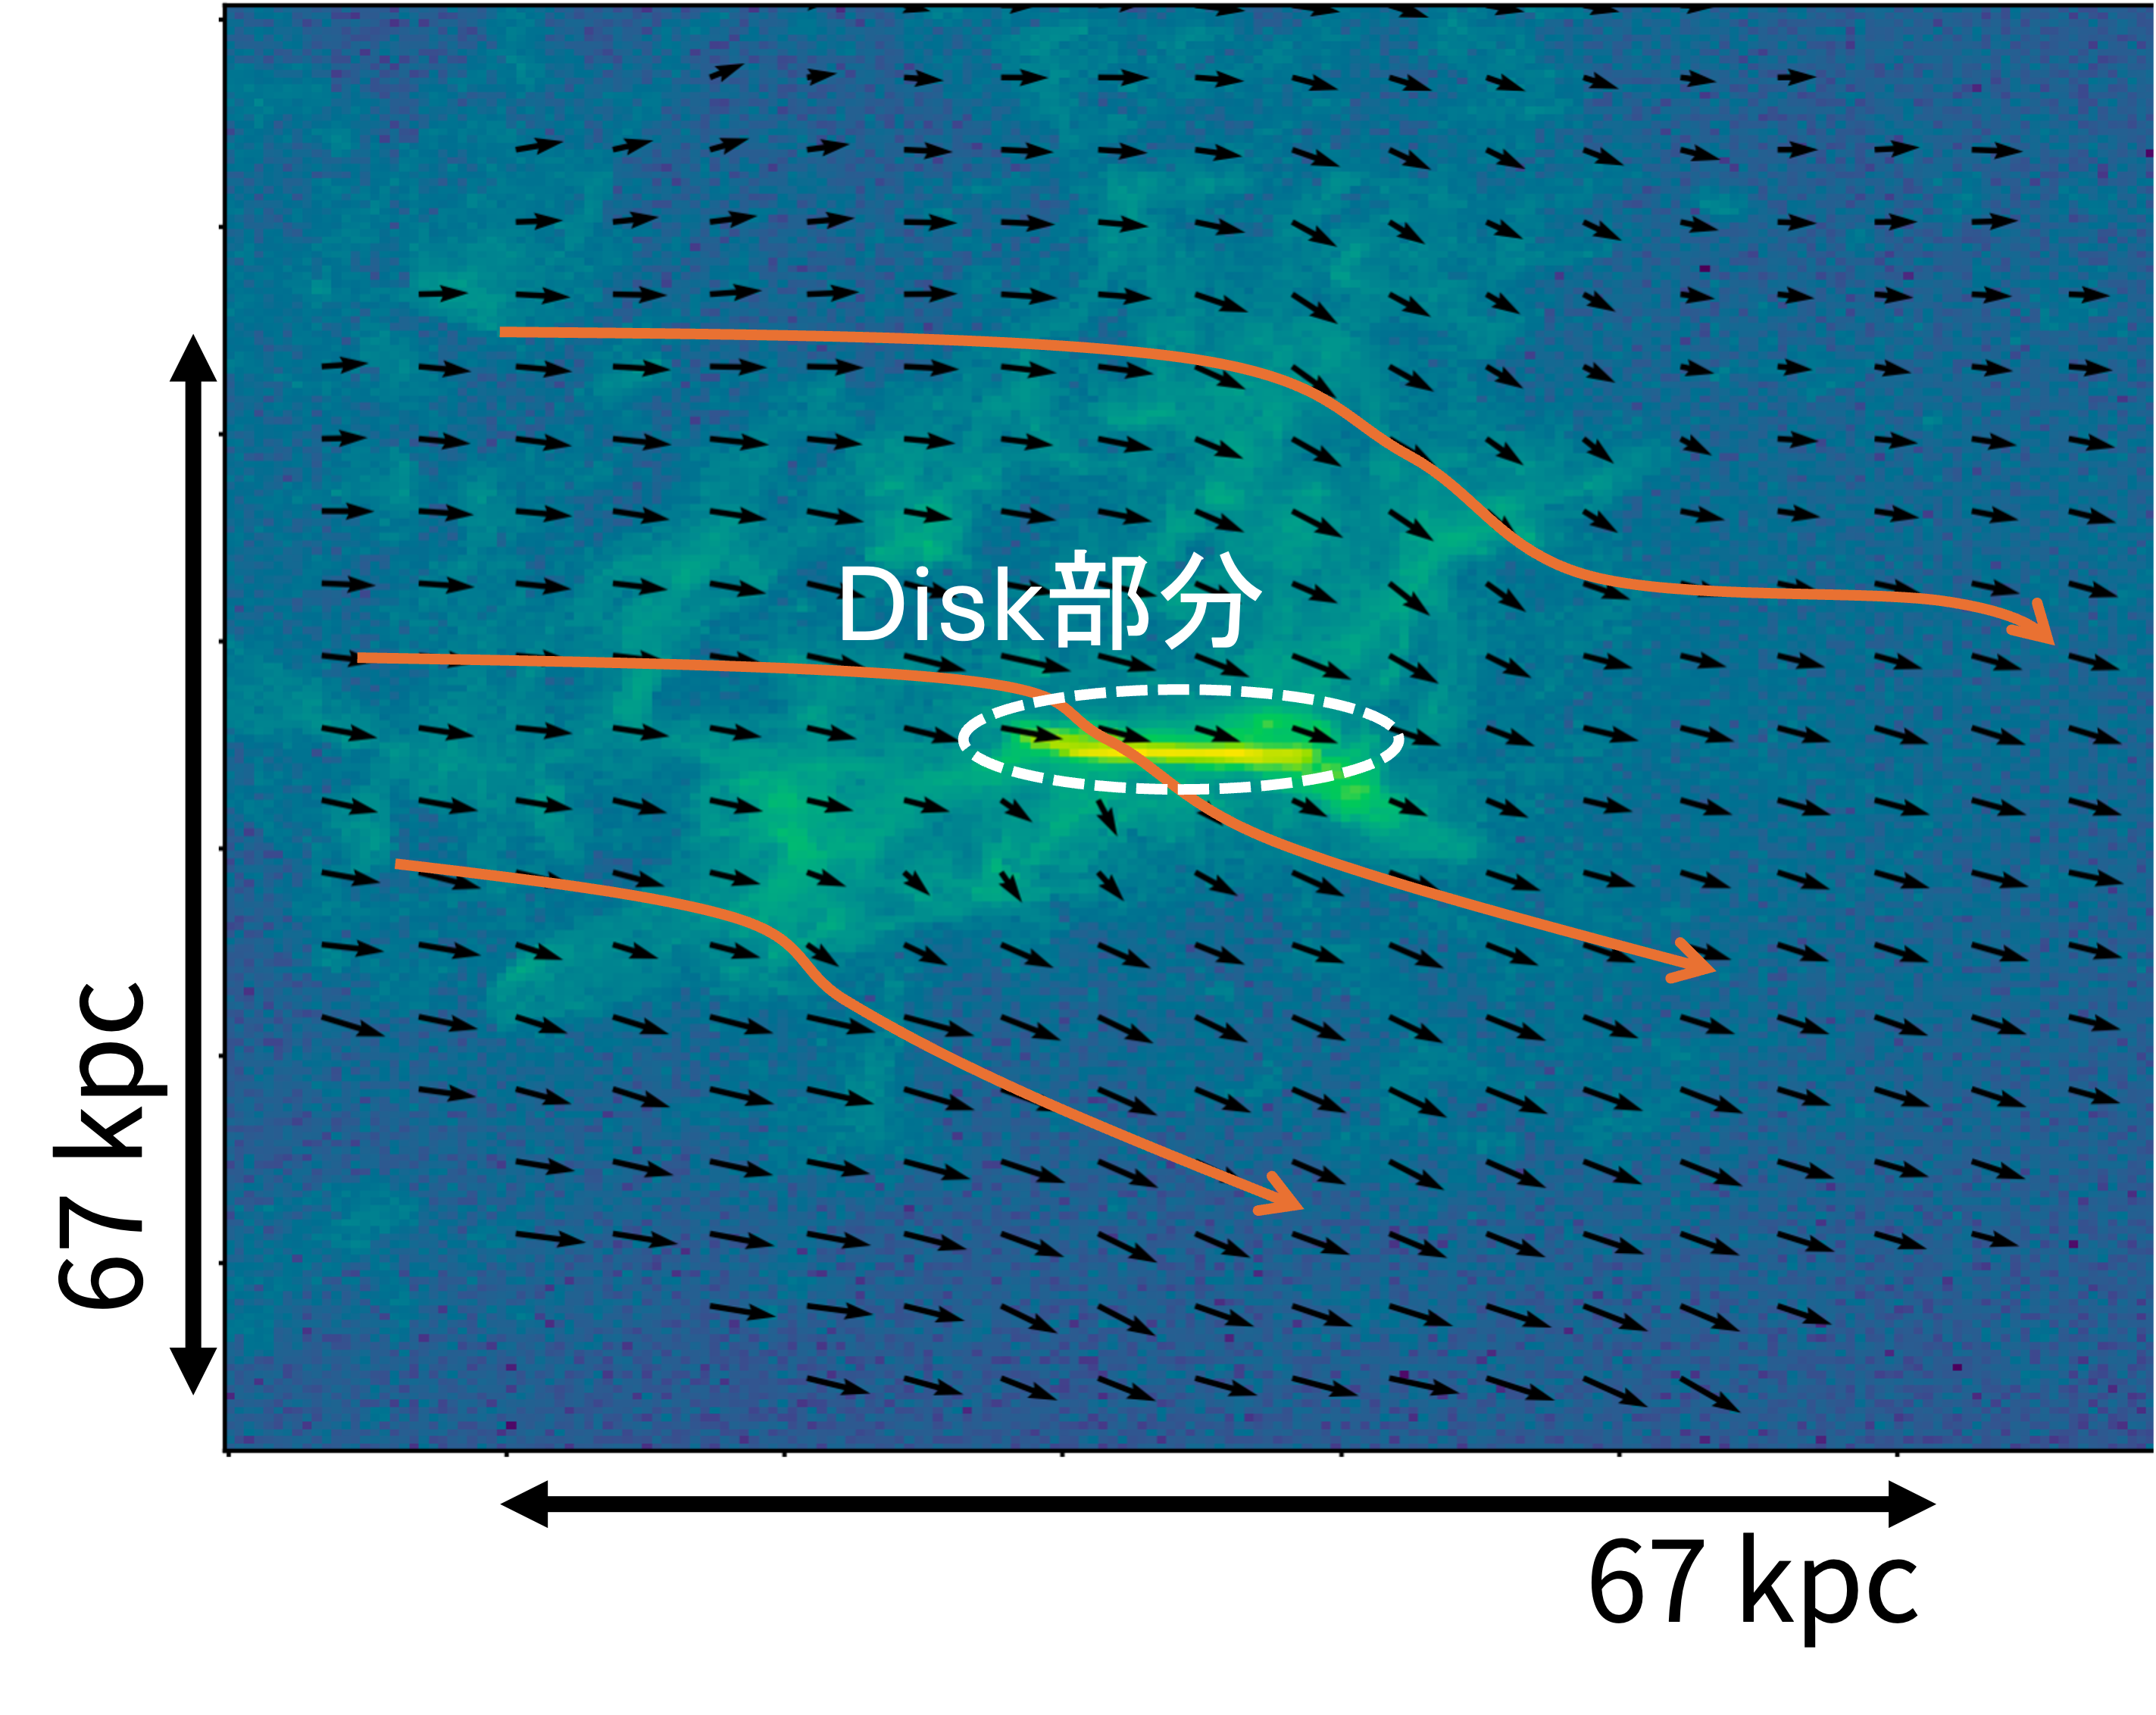
\includegraphics[width=\linewidth]{pic/outflow_subhalo388544}
			\subcaption{subhalo342447}
			\label{fig:outflowsubhalo388544}
		\end{minipage}
		\begin{minipage}[b]{0.45\linewidth}
			\centering
			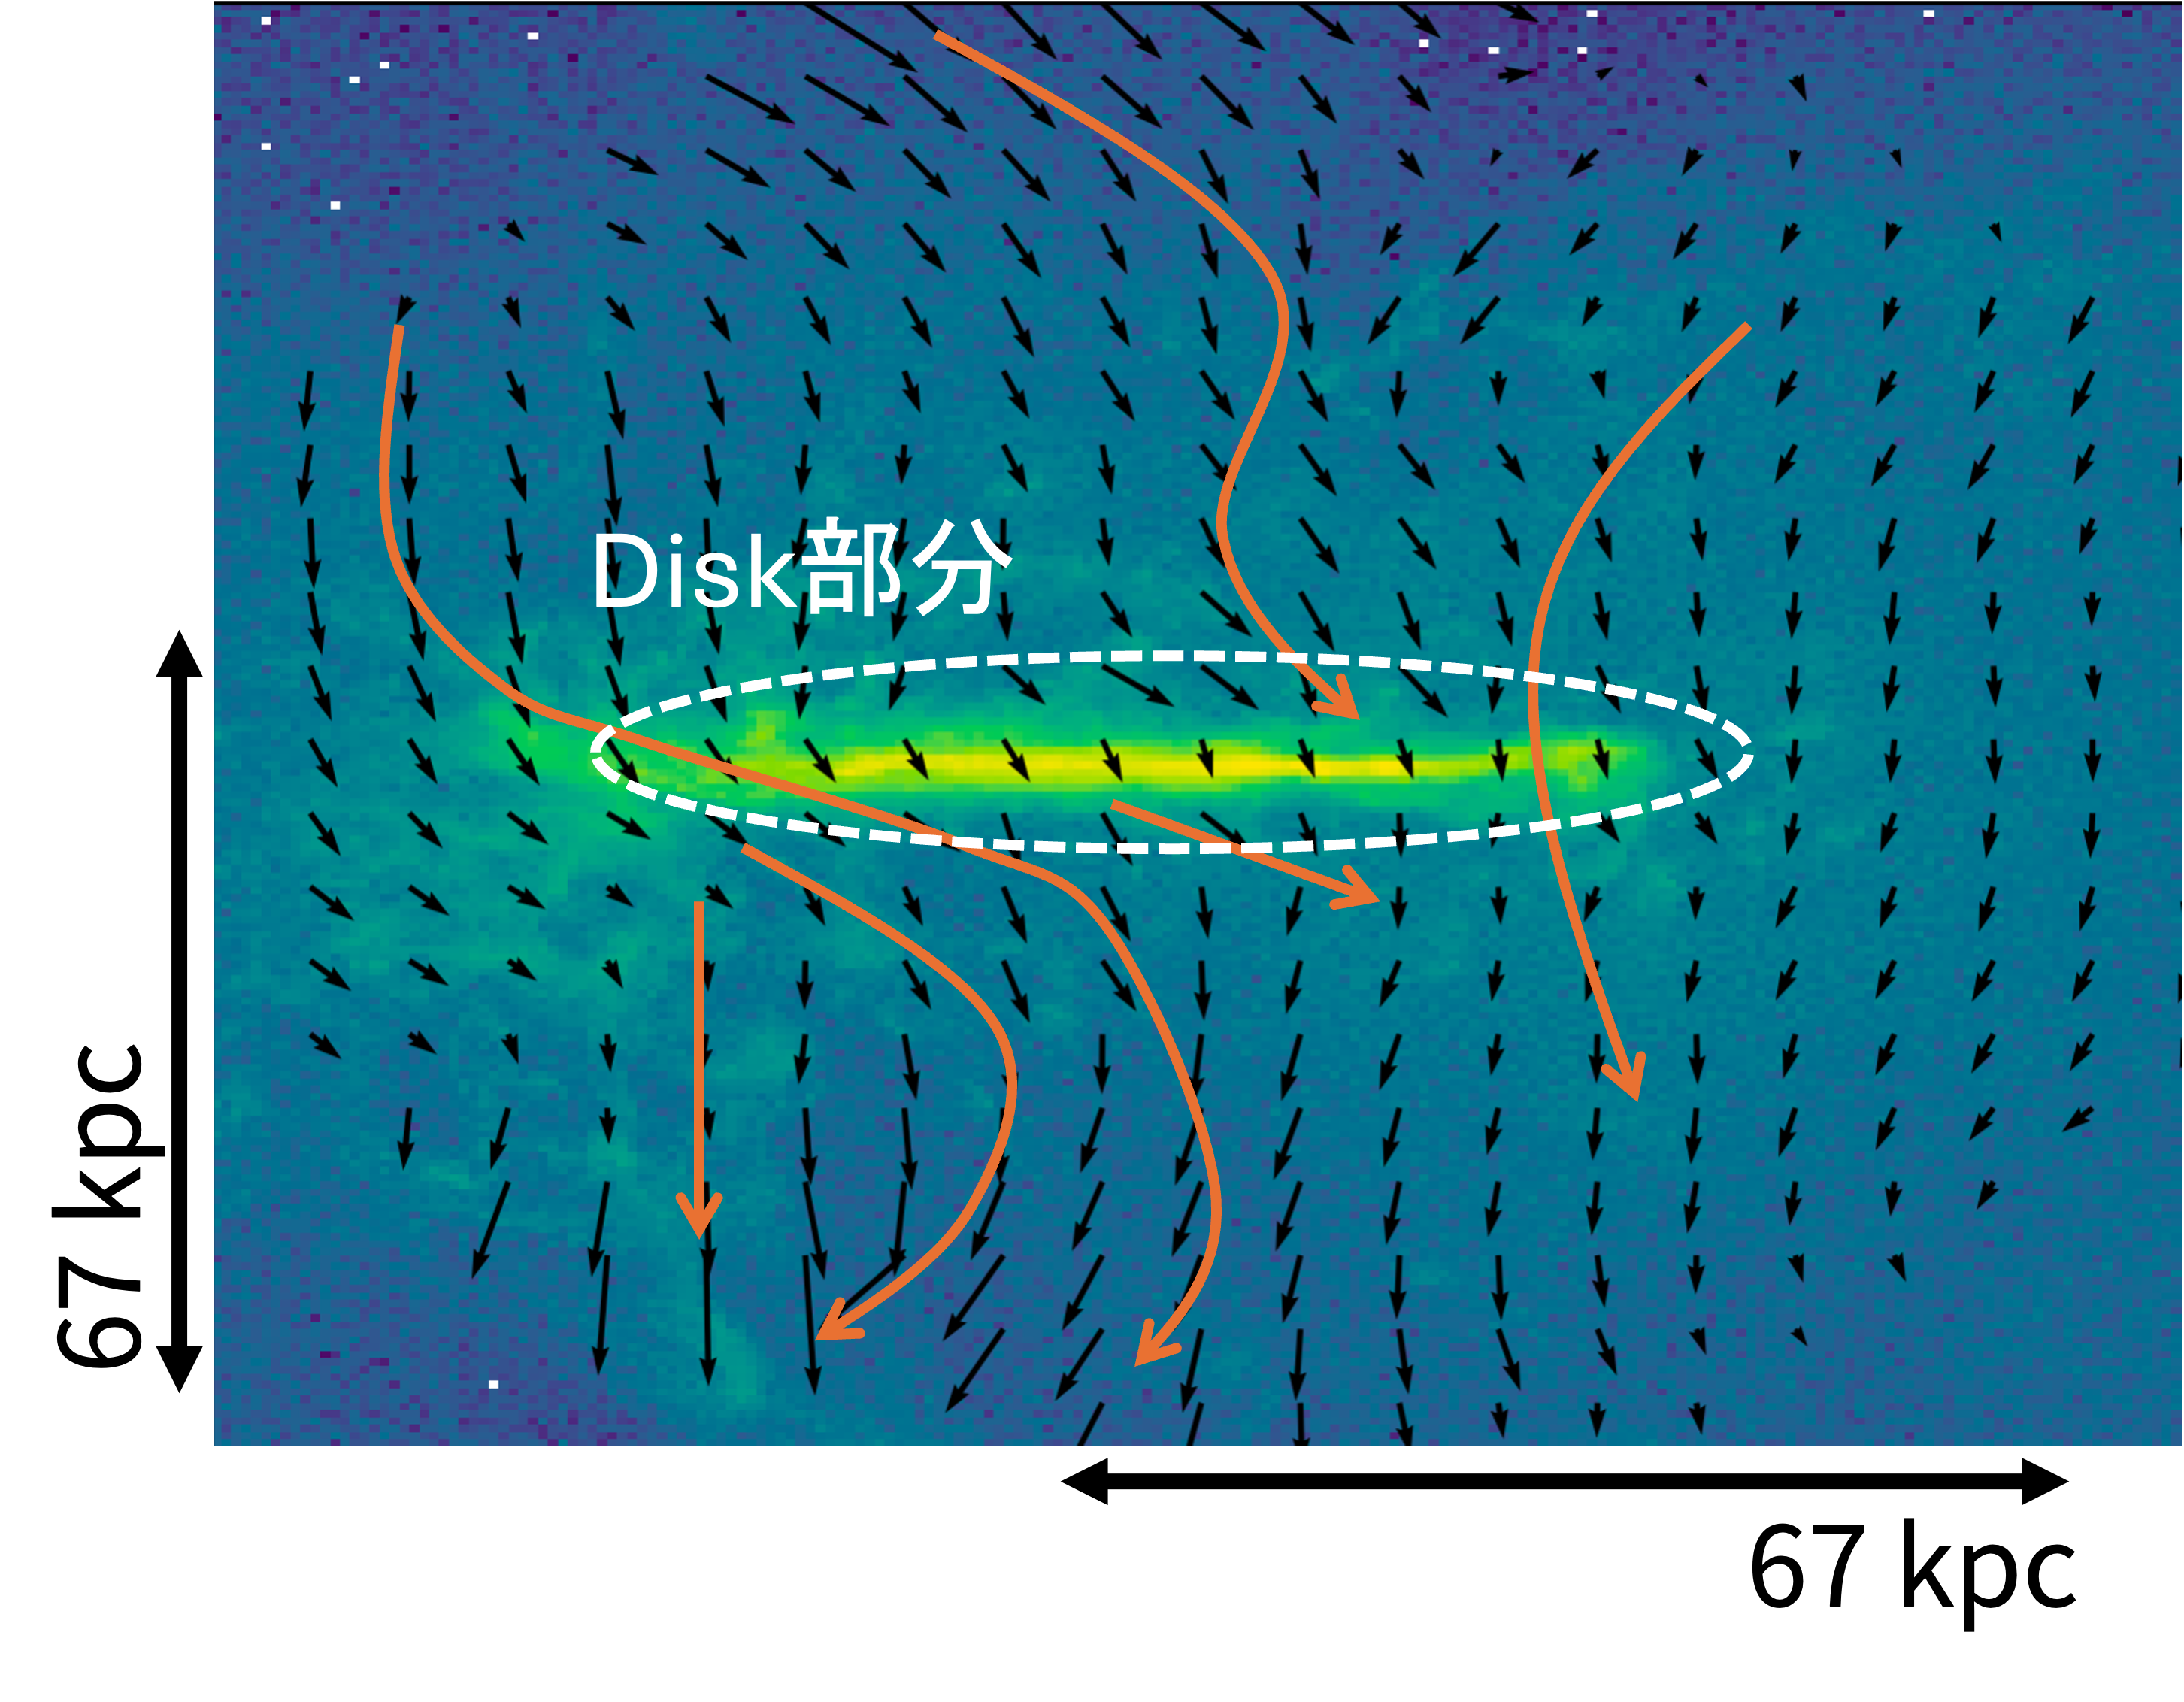
\includegraphics[width=\linewidth]{pic/outflow_subhalo421555}
			\subcaption{subhalo421555}
			\label{fig:outflowsubhalo421555}
		\end{minipage}
		\captionsetup{width=.9\linewidth}
		\caption{edge-onで表示.Massesを背景に表示して速度場を表示している.}
		\label{fig:outflowsubhalo}
	\end{figure}
	
	\section{動径方向の元素分布}
	
	\begin{figure}[htbp]
		\centering
		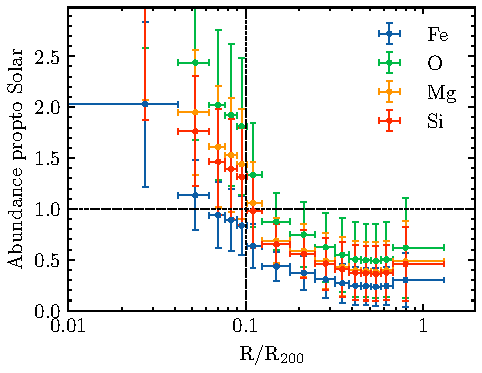
\includegraphics[width=0.7\linewidth]{pic/abundance_profile342447}
		\captionsetup{width=.9\linewidth}
		\caption{subhalo342447}
		\label{fig:abundanceprofile342447}
	\end{figure}
	
	\begin{figure}[htbp]
		\centering
		\begin{minipage}[b]{0.45\linewidth}
			\centering
			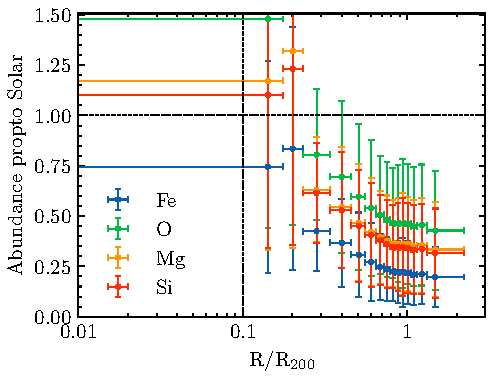
\includegraphics[width=\linewidth]{pic/abundance_profile388544}
			\subcaption{subhalo388544}
			\label{fig:abundanceprofile388544}
		\end{minipage}
		\begin{minipage}[b]{0.45\linewidth}
			\centering
			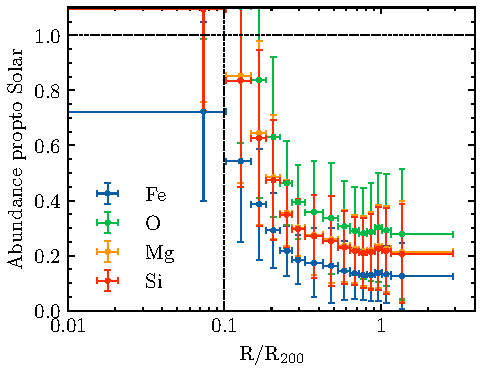
\includegraphics[width=\linewidth]{pic/abundance_profile421555}
			\subcaption{subhalo421555}
			\label{fig:abundanceprofile421555}
		\end{minipage}
		\caption{}
		\label{}
		
	\end{figure}
\end{document}
